%%%%%%%%%%%%%%%%%%%%%%%%%%%%%%%%%%%%%%%%%%%%%%%%%%%%%%%%%%%%%%%%%%%%%%%%%%%%%%%%
%2345678901234567890123456789012345678901234567890123456789012345678901234567890
%        1         2         3         4         5         6         7         8

\documentclass[letterpaper, 10 pt, conference]{ieeeconf}  % Comment this line out
                                                          % if you need a4paper
%\documentclass[a4paper, 10pt, conference]{ieeeconf}      % Use this line for a4
                                                          % paper

\IEEEoverridecommandlockouts                              % This command is only
                                                          % needed if you want to
                                                          % use the \thanks command
\overrideIEEEmargins

\usepackage[english]{babel}
\usepackage[utf8]{inputenc}
\usepackage{amsmath}
\usepackage{graphicx}
\usepackage[colorinlistoftodos]{todonotes}
\usepackage{caption}
\usepackage{subcaption}

\title{\LARGE \bf
Improving Automatic Whiteout++ through Feature Selection
}

\author{Team 3}
%\author{Anurag Kyal, Luke Tornquist, Vinay Kola, and Yuan Ma}

\begin{document}

\maketitle
\thispagestyle{empty}
\pagestyle{empty}
\nocite{*} % Show all Bib-entries

\section{Problem Description}
Mini-QWERTY keyboards are among the most common input technologies for mobile phones in the current generation. BlackBerry Limited along with other companies using mini-QWERTY on their mobile devices have produced a huge user base. These keyboards are of the size of keypads and encompass everything from a normal QWERTY keyboard including space bar and the shift keys.  While touchscreen keyboards are becoming more relevant, physical keyboards are still very much in use and are going to be the focus of this research.

Designs that deploy keyboards with key sizes of $25 mm^{2}$ and inter-key spacing of $2 mm$\cite{clawson2006mobile} are not uncommon. The users’ thumbs being much larger, make visibility difficult and users get adapted to using the keyboard without visual assistance. This results in users making all types of errors like pressing multiple keys at once and pressing an unintended key. Fitts’ Law implies that typing accuracy decreases as typing speed increases due to the relationship between target size, movement speed, and accuracy\cite{soukoreff2004towards}.  Smarter keyboards which can detect and automatically correct such human errors are important not only for a better user experience but also carry a huge business impact.

\section{Related Work}
The most relevant work done in this particular area was done with Automatic Whiteout++.  The main focus of this algorithm was to improve the original design to better detect and correct roll-on, roll-off, key repeat, and row substitution error.  Row subsitution errors account for $45\%$ of the total errors, so targeting and fixing these errors would produce a significant accurance boost\cite{clawson2008automatic}.  The algorithm utilizes decision trees in combination with Weka J48 to learn and classify keystrokes as errors or not.  Some of the common features used in this decision tree are keys pressed, timing information, a letter’s frequency in the English language, and adjacency to other keys.  There were also some newer features added to the algorithm, such as bi-letter/tri-letter frequencies, probability based on large plain-text corpus, and subsequent keypress evaluation.  This allowed for the additional ability to handle row substitution error, and to improve the accuracy of corrections on the original Automatic Whiteout.

With all that being said, the correction accuracy can be further improved by adding some additional features to the decision tree.  Physical limitations of the thumb and fingers while typing can have a great affect on the accuracy of said typing.  This can be classified in a feature and utilized to better train a decision tree to more accurately predict errors while typing.  This was not mentioned in the Automatic Whiteout++ implementation, and should allow for better prediction of typing errors.

\section{Approach}

\subsection{Feature Selection}

Automatic Whiteout++ incorporates 82 features, including bi-gram and tri-gram probabilities of letters and timing of key presses before and after the character in question.

We envisioned two types of features to improve the performance of the error detector.

\subsubsection{Keyboard division}

These features are based on our aim to encode the position of the key on the keyboard. Certain regions could be more conducive to errors due to difficulty of reaching that area. Hence we propose 3 different features for keyboard division:
\begin{itemize}
\item 3X3 rectangular grid
\item Distance of the key from the bottom two corners of the phone to mimic thumb range (\ref{fig:divfeature2})
\item Distance of the key from the default position of the thumb when the phone is held (\ref{fig:divfeature3})
\end{itemize}

\begin{figure}[!h]
    \centering
    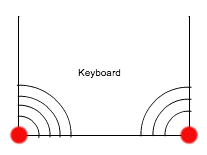
\includegraphics[scale=0.8]{heuristic2.png}
    \caption{Distance from the bottom corners of the keyboard}
    \label{fig:divfeature2}
\end{figure}

\begin{figure}[!h]
    \centering
    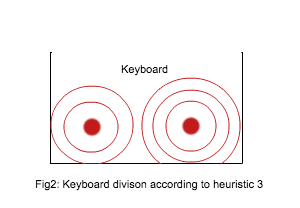
\includegraphics[scale=0.8]{heuristic3.png}
    \caption{Distance from the default position of the thumb}
    \label{fig:divfeature3}
\end{figure}

\subsubsection{Insertion and Substitution probabilities}
Kernighan et al\cite{kernighan1990spelling} computed a set of confusion tables for different types of spelling errors - deletions, insertions, substitutions and transpositions. The tables were computed based on data from the Associated Press (AP) newswire. The ones that are of interest to us are insertions and substitutions. The values in the respective tables denote probability of inserting character $X$ given that the previous character was $Y$ and the probability of substituting character $X$ with $Y$ respectively. 

For each character in the alphabet, we calculate the probability of it being inserted as an error, and the probability of inserting an error character after it using the following formulae:

If insertions$[X,Y]$ = count[inserting $Y$ after $X$],

then we can compute

\begin{align*}
p_{inserted}[X] = \frac{\sum\limits_{X=a}^{z} insertions[X,Y]}{\sum\limits_{X=a}^{z} \sum\limits_{Y=a}^{z}insertions[X,Y]}\\
p_{insert-error-after}[X] = \frac{\sum\limits_{Y=a}^{z} insertions[X,Y]}{\sum\limits_{X=a}^{z} \sum\limits_{Y=a}^{z}insertions[X,Y]}
\end{align*}

Similarly, we can compute the probability of a character being present due to the substitution of the actual correct character as follows:

\begin{align*}
p_{substitution}[X] = \frac{\sum\limits_{Y=a}^{z} substitutions[X,Y]}{\sum\limits_{X=a}^{z} \sum\limits_{Y=a}^{z}substitutions[X,Y]}
\end{align*}

So, for each character we calculate 3 probabilities that we add as features.

\subsection{Algorithm}

Similar to Automatic Whiteout++, we decided to use decision trees to detect the errors. Given the number of features we have, decision trees are a good choice. Specifically, we used the J48 learning algorithm to build the decision tree.

\section{Evaluation}

As Automatic Whiteout++, we used a set of experimental data that is an output of studies on the Dell and the Targus keyboards. The study was carried out with 14 participants and 400 minutes of typing for each. The Twidor software was used to carry out the typing experiment. A total of 42,340 phrases were collected which accounted for 1,261,791 phrases. The data was further processed and each key press was characterised as correct or error. This set of data was used for training and testing.

We randomly separated 10\% of the data to constitute the test set and the remaining 90\% was used to train the model using the new features in conjunction with the old features of Automatic Whiteout++. Again similar to Automatic Whiteout++, we use the Weka J48 decision tree to train and model the data. Three models were built and tested with the same training and test data. While the first is the original Automatic Whiteout++ (we refer it as the baseline), the second and third are the models built by adding the keyboard division feature and then the probability features incrementally. So, the following models were compared:
\begin{itemize}
\item Automatic Whiteout++
\item Automatic Whiteout++ + keyboard division features
\item Automatic Whiteout++ + keyboard division features + substitution and insertion probability features
\end{itemize}

For each of these models, we report their performance on the training set averaged across ten folds (10-fold cross-validation) and then on the test set using the respective trained model in the following 6 tables. Each table has metrics for the four types of the off-by-one error and for each type of error, we report the following metrics:
\begin{itemize}
\item TP: The number of actual errors that were correctly classified
\item FN: The number of actual errors which were incorrectly classified as some other type of error of nonerror
\item FP: The number of nonerrors that were classified as errors
\item TP + TN: Total number of actual errors
\item TP + FP: Total number of errors guessed
\item Precision: Percentage of total classification as errors that were actual errors
\item Recall: Percentage of total actual errors that were correctly classified
\end{itemize}

\begin{table}[h]
\begin{center}
\begin{tabular}{|l|c|c|c|c|c|c|c|} \hline
& TP & TN & FP & TP+TN & TP+FP & Precision & Recall \\ \hline
Roll-on & 2285 & 695 & 692 & 2980 & 2977 & 76.68\% & 76.76\% \\ \hline
Roll-off & 2959 & 154 & 442 & 3113 & 3401 & 95.05\% & 87.00\% \\ \hline
Repeat & 540 & 146 & 193 & 686 & 733 & 78.72\% & 73.67\% \\ \hline
Substitute & 3014 & 954 & 2670 & 3968 & 5684 & 75.96\% & 53.03\% \\ \hline
\end{tabular}
\caption{Baseline - Cross Validation Metrics}
\label{table:basecvm}
\end{center}
\end{table}

\begin{table}[h]
\begin{center}
\begin{tabular}{|l|c|c|c|c|c|c|c|} \hline
& TP & TN & FP & TP+TN & TP+FP & Precision & Recall \\ \hline
Roll-on & 240 & 68 & 71 & 308 & 311 & 77.92\% & 77.17\% \\ \hline
Roll-off & 366 & 13 & 46 & 379 & 412 & 96.57\% & 88.83\% \\ \hline
Repeat & 68 & 13 & 28 & 81 & 96 & 83.95\% & 70.83\% \\ \hline
Substitute & 363 & 116 & 290 & 479 & 653 & 75.78\% & 55.59\% \\ \hline
\end{tabular}
\caption{Baseline - Test Data Metrics}
\label{table:basetdm}
\end{center}
\end{table}

\begin{table}[h]
\begin{center}
\begin{tabular}{|l|c|c|c|c|c|c|c|} \hline
& TP & TN & FP & TP+TN & TP+FP & Precision & Recall \\ \hline
Roll-on & 2286 & 700 & 691 & 2986 & 2977 & 76.56\% & 76.79\% \\ \hline
Roll-off & 2980 & 162 & 421 & 3142 & 3401 & 94.84\% & 87.62\% \\ \hline
Repeat & 540 & 145 & 193 & 685 & 733 & 78.83\% & 73.67\% \\ \hline
Substitute & 3006 & 1002 & 2678 & 4008 & 5684 & 75.00\% & 52.89\% \\ \hline
\end{tabular}
\caption{Division Features - Cross Validation Metrics}
\label{table:divisioncvm}
\end{center}
\end{table}

\begin{table}[h]
\begin{center}
\begin{tabular}{|l|c|c|c|c|c|c|c|} \hline
& TP & TN & FP & TP+TN & TP+FP & Precision & Recall \\ \hline
Roll-on & 242 & 66 & 69 & 308 & 311 & 78.57\% & 77.81\% \\ \hline
Roll-off & 374 & 12 & 38 & 386 & 412 & 96.89\% & 90.78\% \\ \hline
Repeat & 68 & 13 & 28 & 81 & 96 & 83.95\% & 70.83\% \\ \hline
Substitute & 365 & 125 & 288 & 490 & 653 & 74.49\% & 55.90\% \\ \hline
\end{tabular}
\caption{Division Features - Test Data Metrics}
\label{table:divisiontdm}
\end{center}
\end{table}

\begin{table}[h]
\begin{center}
\begin{tabular}{|l|c|c|c|c|c|c|c|} \hline
& TP & TN & FP & TP+TN & TP+FP & Precision & Recall \\ \hline
Roll-on & 2282 & 707 & 695 & 2989 & 2977 & 76.35\% & 76.65\% \\ \hline
Roll-off & 2977 & 166 & 424 & 3143 & 3401 & 94.72\% & 87.53\% \\ \hline
Repeat & 523 & 129 & 210 & 652 & 733 & 80.21\% & 71.35\% \\ \hline
Substitute & 3018 & 1002 & 2666 & 4020 & 5684 & 75.07\% & 53.10\% \\ \hline
\end{tabular}
\caption{All Features - Cross Validation Metrics}
\label{table:allcvm}
\end{center}
\end{table}

\begin{table}[h]
\begin{center}
\begin{tabular}{|l|c|c|c|c|c|c|c|} \hline
& TP & TN & FP & TP+TN & TP+FP & Precision & Recall \\ \hline
Roll-on & 242 & 67 & 69 & 309 & 311 & 78.32\% & 77.81\% \\ \hline
Roll-off & 371 & 14 & 41 & 385 & 412 & 96.36\% & 90.05\% \\ \hline
Repeat & 71 & 16 & 25 & 87 & 96 & 81.61\% & 73.96\% \\ \hline
Substitute & 364 & 127 & 289 & 491 & 653 & 74.13\% & 55.74\% \\ \hline
\end{tabular}
\caption{All Features - Test Data Metrics}
\label{table:alltdm}
\end{center}
\end{table}

\section{Discussion}

\bibliographystyle{plain}
\bibliography{main}

\end{document}